\chapter{Fourieranalysis}
\setcounter{section}{12}
\setcounter{subsection}{-1}
\setcounter{subsubsection}{-1}
\setcounter{secnumdepth}{4}
\subsection{Einführung in die Fourieranalysis}
\href{https://youtu.be/7Dge4dbGn78}{Video 01}\\
$\bullet\;\;$Taylorapproximation\\
\begin{quote}
	Mittels der Taylorapproximationen werden diffbare Funktionen mittels Polynome lokal in der Nähe von $ x_0 $ approximieren.\\


\begin{center}
		$ f(x)=\ln(x) \approx \mathrm{T}_{n,x_0}$ \\
	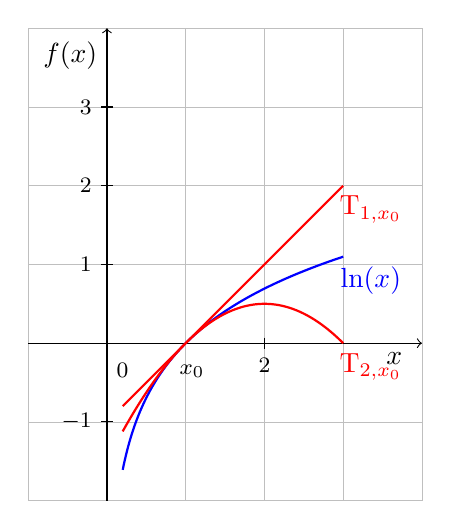
\begin{tikzpicture}[xscale=1, yscale=1]
	
	% Gitternetzlinien
	\draw[xstep=1cm, ystep=1cm, very thin, color=lightgray] (-1,4) grid (4,-2);
	% x-Achse
	\draw[->] (-1,0) -- (4,0) node[below,xshift=-1em] {$x$}; 
	%Zahlen auf x-Achse
	%\foreach \x in {-3,...,-1}
	%\draw[shift={(\x,0)},color=black] (0pt,2pt) -- (0pt,-2pt) node[below] {\footnotesize $\x$};
	\foreach \x in {2,...,2}
	\draw[shift={(\x,0)},color=black] (0pt,2pt) -- (0pt,-2pt) node[below] {\footnotesize $\x$};
	% y-Achse 
	\draw[->] (0,-2) -- (0,4) node[left,yshift=-1em] {$f(x)$};%node[above left]
	%Zahlen auf y-Achse
	\foreach \y in {-1,...,-1}
	\draw[shift={(0,\y)},color=black] (2pt,0pt) -- (-2pt,0pt) node[left] {\footnotesize $\y$};
	\foreach \y in {1,...,3}
	\draw[shift={(0,\y)},color=black] (2pt,0pt) -- (-2pt,0pt) node[left] {\footnotesize $\y$};
	%Ursprung
	\draw[color=black] (0pt,-10pt) node[right] {\footnotesize $0$};
	
\draw[color=black] (0.8,-10pt) node[right] {\footnotesize $x_0$};
	
	\draw[thick,color=blue] plot[samples=200, domain=0.2:3] 
	(\x,{ln(\x)}) node[below, xshift=1em]{$\ln(x)$};
	
	\draw[thick,color=red] plot[samples=200, domain=0.2:3] 
	(\x,{\x-1}) node[below, xshift=1em]{$\mathrm{T}_{1,x_0}$};
		\draw[thick,color=red] plot[samples=200, domain=0.2:3] 
	(\x,{\x-1-0.5*(\x-1)^2}) node[below, xshift=1em]{$\mathrm{T}_{2,x_0}$};
	
	\end{tikzpicture}\\
	
\end{center}
\end{quote}
$\bullet\;\;$Fourieranalysis\\
\begin{quote}
	Mittels der Fourieranalysis werden periodische Funktionen mittels Sinus und Cosinus global approximiert.\\
	\begin{center}
	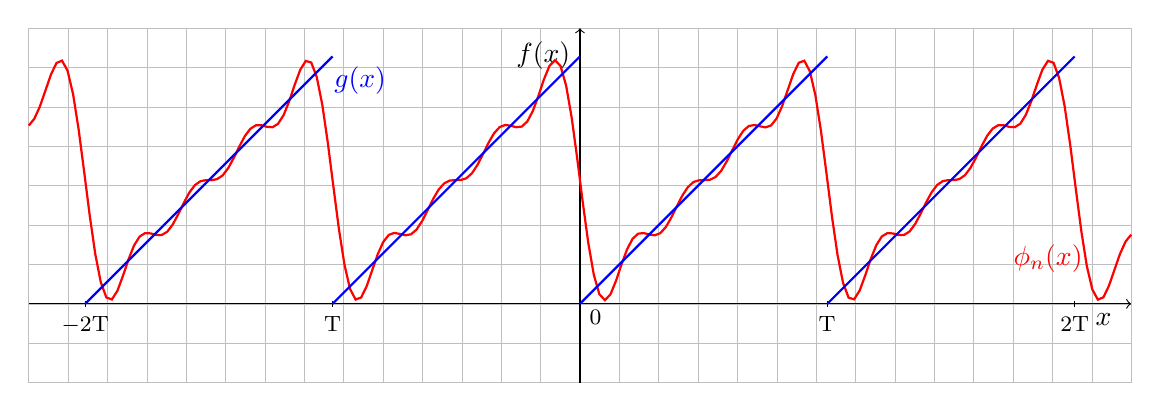
\begin{tikzpicture}[xscale=0.5, yscale=0.5]
	
	% Gitternetzlinien
	\draw[xstep=1cm, ystep=1cm, very thin, color=lightgray] (-14,7) grid (14,-2);
	% x-Achse
	\draw[->] (-14,0) -- (14,0) node[below,xshift=-1em] {$x$}; 
	%Zahlen auf x-Achse
	%\foreach \x in {-3,...,-1}
	%\draw[shift={(\x,0)},color=black] (0pt,2pt) -- (0pt,-2pt) node[below] {\footnotesize $\x$};
	%\foreach \x in {1,...,3}
	%\draw[shift={(\x,0)},color=black] (0pt,2pt) -- (0pt,-2pt) node[below] {\footnotesize $\x$};
	% y-Achse 
	\draw[->] (0,-2) -- (0,7) node[left,yshift=-1em] {$f(x)$};%node[above left]
	%Zahlen auf y-Achse
	%\foreach \y in {-1,...,-1}
	%\draw[shift={(0,\y)},color=black] (2pt,0pt) -- (-2pt,0pt) node[left] {\footnotesize $\y$};
	%\foreach \y in {1,...,3}
	%\draw[shift={(0,\y)},color=black] (2pt,0pt) -- (-2pt,0pt) node[left] {\footnotesize $\y$};
	%Ursprung
	\draw[color=black] (0pt,-10pt) node[right] {\footnotesize $0$};
	

	\draw[shift={(6.28,0)},color=black] (0pt,2pt) -- (0pt,-2pt) node[below] {\footnotesize $\mathrm{T}$};
	\draw[shift={(-2*pi,0)},color=black] (0pt,2pt) -- (0pt,-2pt) node[below] {\footnotesize $\mathrm{T}$};
	
	\draw[shift={(-4*pi,0)},color=black] (0pt,2pt) -- (0pt,-2pt) node[below] {\footnotesize $-2\mathrm{T}$};
	\draw[shift={(4*pi,0)},color=black] (0pt,2pt) -- (0pt,-2pt) node[below] {\footnotesize $2\mathrm{T}$};
	\draw[thick,color=red] plot[samples=200, domain=-14:14] 
	(\x,{pi-2*(sin(\x r)+0.5*sin((2*\x )r)+0.33*sin((3*\x )r)+0.25*sin((4*\x )r)) }) node[below, xshift=-3em]{$\phi_n(x)$};
	
		\draw[thick,color=blue] plot[samples=200, domain=0:2*pi] 
	(\x,{\x } );
		\draw[thick,color=blue] plot[samples=200, domain=2*pi:4*pi] 
	(\x,{\x-2*pi } );
		\draw[thick,color=blue] plot[samples=200, domain=-2*pi:0] 
	(\x,{\x +2*pi} );
	 	\draw[thick,color=blue] plot[samples=200, domain=-4*pi:-2*pi] 
	 (\x,{\x +4*pi} ) node[below, xshift=1em]{$g(x)$};
	\end{tikzpicture}\\	
	\end{center}
Die Funktion $ g(x)=x $, die  um T immer wieder periodisch wiederholt wird kann mittels einer periodischen Funktion $\phi_n(x)$ approximiert werden.\\
\end{quote}
Definition (Periodizität):\\
Eine Funktion hat die Periode T mit $ \mathrm{T}>0 $, wenn gilt:\\
\begin{align*}
f(x+T)=f(x)\;\;\text{ für alle}\; x
\end{align*}
Dann nennet man auch $ f $: T-periodisch.
\\
\\
Beispiel:\\
Der Sinus und der Cosinus sind $2\pi$-periodisch, denn es gilt:\\
\begin{align*}
\sin(x+2\pi)=\sin(x)&&\cos(x+2\pi)=\cos(x)
\end{align*}
Der Sinus und der Cosinus sind $4\pi$-periodisch, denn es gilt:\\
\begin{align*}
\sin(x+2\pi+2\pi)=\sin(x+2\pi)=\sin(x)&&\cos(x+2\pi+2\pi)=\cos(x+2\pi)=\cos(x)
\end{align*}
Allgemein gilt dann: Der Sinus und Cosinus sind $ k2\pi $-periodisch für $ k\in\mathbb{N}\setminus \{0\} $\\
\\
Betrachte: $ \mathrm{T}=\frac{2\pi}{\omega} $\\
Dann sind $ \sin(k\omega x) $ und $\cos( k\omega x) $ T-periodisch.\\
Es gilt:\\
\begin{align*}
\sin(k\omega(x+\mathrm{T}))&=\sin (k\omega x+k\omega \mathrm{T})\;\;\arrowvert\text{\tiny $\mathrm{T}=\frac{2\pi}{\omega} $ }\\
&=\sin (k\omega x+k2\pi)=\sin (k\omega x) \;\;\text{für }\;k\in \mathbb{Z}\\
&\Rightarrow \text{ T-periodisch}
\end{align*}
Bemerkung:\\
Die Funktion $ \sin(k\omega x) $ ist für $ k=1 $ die Grundschwingung.\\
Für $ k=2,3,4... $ enstehen somit alle Oberschwingungen. Diese Funktionen: $ \sin(k\omega x)$ und $ \cos(k\omega x)  $ sind dann die Grundbausteine für die Fourieranalysis.\\
\\
Ebenfalls gilt:\\
\begin{align*}
\mathrm{e}^{\mathrm{i}x}=\cos (x)+\mathrm{i}\sin (x)
\end{align*}
Dann ist die Euler-Form auch T-periodisch:\\
\begin{align*}
\mathrm{e}^{\mathrm{i}k\omega x}= \cos(k\omega x)+\mathrm{i}\sin(k\omega x)
\end{align*}
\newpage
\noindent
\subsection{ Das reelle Fourierpolynom}
\href{https://youtu.be/kBD9vmv_Gio}{Video 02}\\
Sei $ f:\vee\longmapsto\mathbb{R} $ oder $  \mathbb{C} $ eine T-periodische Funktion und stückweise monoton.\\
\begin{center}
Jeder Teilbereich ist monoton\\
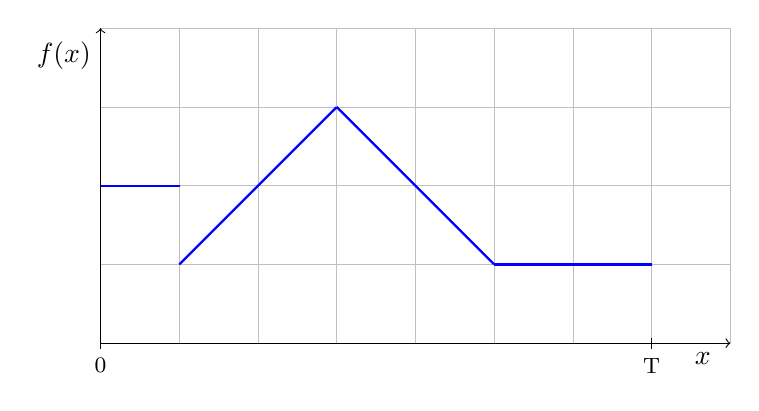
\begin{tikzpicture}[xscale=1, yscale=1]

% Gitternetzlinien
\draw[xstep=1cm, ystep=1cm, very thin, color=lightgray] (0,4) grid (8,0);
% x-Achse
\draw[->] (0,0) -- (8,0) node[below,xshift=-1em] {$x$}; 
%Zahlen auf x-Achse
%\foreach \x in {-3,...,-1}
%\draw[shift={(\x,0)},color=black] (0pt,2pt) -- (0pt,-2pt) node[below] {\footnotesize $\x$};
%\foreach \x in {1,...,3}
%\draw[shift={(\x,0)},color=black] (0pt,2pt) -- (0pt,-2pt) node[below] {\footnotesize $\x$};
% y-Achse 
\draw[->] (0,0) -- (0,4) node[left,yshift=-1em] {$f(x)$};%node[above left]
%Zahlen auf y-Achse
%\foreach \y in {-1,...,-1}
%\draw[shift={(0,\y)},color=black] (2pt,0pt) -- (-2pt,0pt) node[left] {\footnotesize $\y$};
%\foreach \y in {1,...,3}
%\draw[shift={(0,\y)},color=black] (2pt,0pt) -- (-2pt,0pt) node[left] {\footnotesize $\y$};
%Ursprung

\draw[shift={(7,0)},color=black] (0pt,2pt) -- (0pt,-2pt) node[below] {\footnotesize $\mathrm{T}$};
\draw[shift={(0,0)},color=black] (0pt,2pt) -- (0pt,-2pt) node[below] {\footnotesize $\mathrm{0}$};
\draw[thick,color=blue] plot[samples=200, domain=0:1] 
(\x,{2});
\draw[thick,color=blue] plot[samples=200, domain=1:3] 
(\x,{\x});

\draw[thick,color=blue] plot[samples=200, domain=3:5] 
(\x,{-\x+6});
\draw[thick,color=blue] plot[samples=200, domain=5:7] 
(\x,{1});
\end{tikzpicture}\\	

\end{center}
Sei $ \omega =\frac{2\pi}{T} $, dann definieren wir für $ k\in\mathbb{N} $ die Fourierkoeffizienten durch:\\
\begin{center}
	\fbox{\parbox  {50mm} {$a_0=\frac{2}{T}\int\limits_{0}^{\mathrm{T}}f(x)\mathrm{d}x \\a_k=\frac{2}{\mathrm{T}}\int\limits_{0}^{\mathrm{T}}f(x)\cos(k\omega x)\mathrm{d}x   $\\ $b_k=\frac{2}{\mathrm{T}}\int\limits_{0}^{\mathrm{T}}f(x)\sin(k\omega x)\mathrm{d}x   $}}
\end{center}
Dann ist das n-Fourierpolynom (n-ter Ordnung) von der Form:\\
\begin{center}
\boxed{ \phi_n(x)=\frac{a_0}{2} +\sum\limits_{k=1}^{n}a_k\cos(k\omega x)+b_k\sin(k\omega x)}	
\end{center}
Nach der Approximation gilt dann:\\
\begin{align*}
&f(x)\approx \phi_n(x)\\
&f(x)=\lim\limits_ {n\to\infty}\phi_n(x)
\end{align*}
\addtocounter{subsubsection}{1}
\subsubsection{ Beispiel zum reellen Fourierpolynom}
\href{https://youtu.be/EsfssnLs8To}{Video 03}\\
Berachte die T-periodische Funktion $ f(x)=\cos(x)+2\sin(x) $ mit $ 2\pi=\mathrm{T}=\frac{2\pi}{\omega} $ und berechne das 1.-Fourierpolynom.\\
Bemerkung:\\
\begin{align*}
\text{für } \omega=1 \;\;\text{gilt: } \mathrm{T}=\frac{2\pi}{\omega}\Rightarrow \mathrm{T}=2\pi
\end{align*}
Es gilt:\\
\begin{align*}
& \phi_n(x)=\frac{a_0}{2} +\sum\limits_{k=1}^{n}a_k\cos(k\omega x)+b_k\sin(k\omega x)\\
&\text{mit }\;\;\omega=1 \;\;\text{und }\;\;k=1\;\;\text{ergibt sich das 1.-Fourierpolynom: }\\
& \phi_n(x)=\frac{a_0}{2} +a_1\cos(x)+b_1\sin( x)\\
\end{align*}
\underline{Berechnung von $ a_0 $:}\\
\begin{align*}
a_0&=\frac{2}{T}\int\limits_{0}^{\mathrm{T}}f(x)\mathrm{d}x\\
&=\frac{2}{2\pi}\int\limits_{0}^{2\pi} \cos(x)+2\sin(x)\mathrm{d}x\\
&=\frac{1}{\pi}\bigg[\sin(x)-2\cos(x)\bigg]^{2\pi}_0\\
&=\frac{1}{\pi}\bigg(\sin(2\pi)-2\cos(2\pi)-\big(\sin(0)-2\cos(0)\big)\bigg)\\
a_0&=\frac{1}{\pi}\cdot0=0
\end{align*}
Bemerkung:\\
Das Integral von $ \cos(x), \sin(x) $ mit den Grenzen über genau einer Periode ergibt die Fläche: A=0.\\
\begin{center}
	
Fläche A=0\\
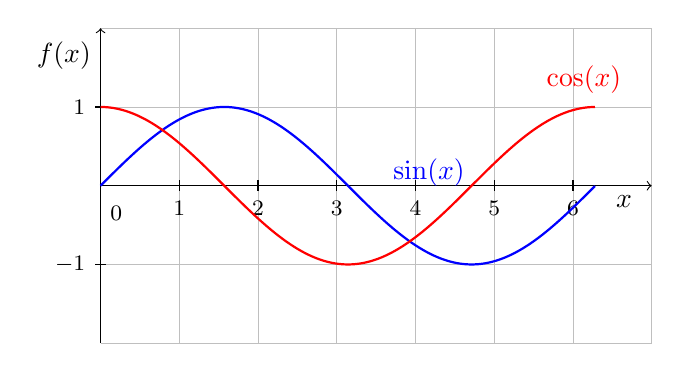
\begin{tikzpicture}[xscale=1, yscale=1]

% Gitternetzlinien
\draw[xstep=1cm, ystep=1cm, very thin, color=lightgray] (0,2) grid (7,-2);
% x-Achse
\draw[->] (0,0) -- (7,0) node[below,xshift=-1em] {$x$}; 
%Zahlen auf x-Achse
%\foreach \x in {-3,...,-1}
%\draw[shift={(\x,0)},color=black] (0pt,2pt) -- (0pt,-2pt) node[below] {\footnotesize $\x$};
\foreach \x in {1,...,6}
\draw[shift={(\x,0)},color=black] (0pt,2pt) -- (0pt,-2pt) node[below] {\footnotesize $\x$};
% y-Achse 
\draw[->] (0,-2) -- (0,2) node[left,yshift=-1em] {$f(x)$};%node[above left]
%Zahlen auf y-Achse
\foreach \y in {-1,...,-1}
\draw[shift={(0,\y)},color=black] (2pt,0pt) -- (-2pt,0pt) node[left] {\footnotesize $\y$};
\foreach \y in {1,...,1}
\draw[shift={(0,\y)},color=black] (2pt,0pt) -- (-2pt,0pt) node[left] {\footnotesize $\y$};
%Ursprung
\draw[color=black] (0pt,-10pt) node[right] {\footnotesize $0$};

\draw[thick,color=blue] plot[samples=200, domain=0:6.28] 
(\x,{sin(\x r) }) node[ xshift=-6em,yshift=5] {$\sin(x)$};

\draw[thick,color=red] plot[samples=200, domain=0:6.28] 
(\x,{cos(\x r}) node[ yshift=1em,xshift=-4]{$\cos(x)$};


\end{tikzpicture}\\

	
\end{center}
\underline{Berechnung von $ a_1 $:}\\
\begin{align*}
a_1&=\frac{2}{2\pi}\int\limits_{0}^{\mathrm{2\pi}}f(x)\cos( x)\mathrm{d}x  \\
&=\frac{1}{\pi}\int\limits_{0}^{2\pi} \big(\cos(x)+2\sin(x)\big)\cos(x)\mathrm{d}x\\
&=\frac{1}{\pi}\int\limits_{0}^{2\pi} \big(\cos^2(x)+2\sin(x)\cos(x)\big)\mathrm{d}x\\
\end{align*}
\\
\\
\\
\\
\\
\\
\begin{quote}
NR.: Stammfunktionen von $ \int\limits_{}^{}\big(\cos(x)\sin(x)\big) \mathrm{d}x $ und $ \int\limits_{}^{} \cos^2(x)\mathrm{d}x $ bestimmen.\\
	$ \bullet\;\;  \int\limits_{}^{}\big(\cos(x)\sin(x)\big)\mathrm{d}x$ (Substitution)
	\begin{align*}
	&\int\limits_{}^{}\big(\cos(x)\sin(x)\big)\mathrm{d}x\\
	&u=\sin(x)\\
	&\frac{\mathrm{d}u}{\mathrm{d}x}=\frac{\sin(x)}{\mathrm{dx}}=\cos(x)\\
	&\Leftrightarrow \mathrm{d}x=\frac{du}{\cos(x)}\\
	&\Rightarrow\\
	&\int\limits_{}^{} \big(\sin(x)\cos(x)\big)\mathrm{d}x=\int\limits_{}^{} u \cdot \cos(x)\frac{\mathrm{d}u}{\cos(x)}=\int\limits_{}^{} u\cdot \mathrm{d}u=\frac{1}{2}u^2\\
	&\text{Rücksubstitution: }\;u=\sin(x)\\
	&\int\limits_{}^{} \big(\sin(x)\cos(x)\big)\mathrm{d}x=\frac{1}{2}\sin^2(x)+\mathrm{c}
	\end{align*}
		$ \bullet\;\;  \int\limits_{}^{}\cos^2(x)\mathrm{d}x$ (Partialintegration)\\
		\begin{align*}
		&\int\limits_{}^{} \cos^2(x)\mathrm{d}x=\int\limits_{}^{} \big(\cos(x)\cos(x)\big)\mathrm{d}x\\
		&u=\cos(x)\Rightarrow u'=-\sin(x)\\
		&v'=\cos(x)\Rightarrow v=\sin(x)\\
		&\int\limits_{}^{} \cos^2(x)\mathrm{d}x=\cos(x)\cdot \sin(x)-\int\limits_{}^{} -\sin(x)^2(x)\mathrm{d}x\;\;\arrowvert\text{\tiny $ \cos^2(x)+\sin^2(x)=1\Leftrightarrow \sin^2(x)=1-\cos^2(x) $ }\\
		&\int\limits_{}^{} \cos^2(x)\mathrm{d}x=\cos(x)\sin(x)+\int\limits_{}^{} \big(1-\cos^2(x)\big)\mathrm{d}x\\
		&\int\limits_{}^{} \cos^2(x)\mathrm{d}x=\cos(x)\sin(x)+\int\limits_{}^{} 1\mathrm{d}x-\int\limits_{}^{} \cos^2(x)\mathrm{d}x\\
		\Leftrightarrow&2\int\limits_{}^{} \cos^2(x)\mathrm{d}x=\cos(x)\sin(x)+x\\
		\Leftrightarrow&\int\limits_{}^{} \cos^2(x)\mathrm{d}x=\frac{1}{2}\big(x+\cos(x)\sin(x)\big)+\mathrm{c}\\
		&\text{Es gilt: }\;\;\sin(x+x)=\sin(x)\cos(x)+\sin(x)\cos(x)\;\;|\text{ \tiny Additiontheorem}\\
		&\sin(2x)=2\sin(x)\cos(x)\\
		&\Leftrightarrow \cos(x)\sin(x)=\frac{1}{2}\sin(2x)\\
		&\text{Dies eingesetzt ergibt dann die Stammfunktion: }\\
		&\int\limits_{}^{} \cos^2(x)\mathrm{d}x=\frac{1}{2}\bigg(x+\frac{1}{2}\sin(2x)\bigg)+\mathrm{c}\\
		\end{align*}
\end{quote}
Nun weiter mit der Berechnung von $ a_1 $:\\
\begin{align*}
a_1&=\frac{1}{\pi}\int\limits_{0}^{2\pi} \big(\cos^2(x)+2\sin(x)\cos(x)\big)\mathrm{d}x\\
&=\frac{1}{\pi}\bigg[\frac{x}{2}+\frac{\sin(2x)}{4}+\sin^2(x)\bigg]^{2\pi}_0\\
&=\frac{1}{\pi}\big(\pi+0-(0)\big)=\frac{\pi}{\pi}=1\\
a_1&=1
\end{align*}
\underline{ Berechnung von $ b_1 $:}\\
\begin{align*}
b_1&=\frac{2}{2\pi}\int\limits_{0}^{\mathrm{2\pi}}f(x)\sin( x)\mathrm{d}x  \\
&=\frac{1}{\pi}\int\limits_{0}^{2\pi} \big(\cos(x)+2\sin(x)\big)\sin(x)\mathrm{d}x\\
&=\frac{1}{\pi}\int\limits_{0}^{2\pi} \big(\cos(x)\sin(x)+2\sin^2(x)\big)\mathrm{d}x\\
\end{align*}
\begin{quote}
NR.: Stammfunktionen von $ \int\limits_{}^{}\sin^2(x) \mathrm{d}x $ bestimmen.\\
\begin{align*}
&\int\limits_{}^{} \sin(x)\sin(x)\mathrm{d}x\\
&u=\sin(x)\Rightarrow u'=\cos(x)\\
&v'=\sin(x)\Rightarrow v=-\cos(x)\\
&\int\limits_{}^{} \sin^2(x)\mathrm{d}x=\sin(x)\cdot -\cos(x)-\int\limits_{}^{} -\cos^2(x)\mathrm{d}x\;\;\lvert\text{\tiny $\cos^2(x)+\sin^2(x)=1\Leftrightarrow \cos^2(x)=1-\sin^2(x)$ }\\
&\int\limits_{}^{} \sin^2(x)\mathrm{d}x=-\sin(x)\cos(x)+\int\limits_{}^{} 1-\sin^2(x)\mathrm{d}x\\
&\int\limits_{}^{} \sin^2(x)\mathrm{d}x=-\sin(x)\cos(x)+\int\limits_{}^{} 1\mathrm{d}x-\int\limits_{}^{} \sin^2(x)\mathrm{d}x\\
\Leftrightarrow&2\int\limits_{}^{} \sin^2(x)\mathrm{d}x=-\sin(x)\cos(x)+x\\
\Leftrightarrow&\int\limits_{}^{} \sin^2(x)\mathrm{d}x=\frac{1}{2}\big(x-\sin(x)\cos(x)\big)\;\;\text{\tiny$\cos(x)\sin(x)=\frac{1}{2}\sin(2x)  $ }\\
&\int\limits_{}^{} \sin^2(x)\mathrm{d}x=\frac{1}{2}\bigg(x-\frac{1}{2}\sin(2x)\bigg)+\mathrm{c}
\end{align*}
\end{quote}
Nun weiter mit der Berechnung von $ b_1 $:\\
\begin{align*}
&=\frac{1}{\pi}\int\limits_{0}^{2\pi} \big(\cos(x)\sin(x)+2\sin^2(x)\big)\mathrm{d}x\\
&=\frac{1}{\pi}\bigg[\frac{1}{2}\sin^2(x)+2\bigg(\frac{x}{2}-\frac{\sin(2x)}{4}\bigg)\bigg]^{2\pi}_0\\
&=\frac{1}{\pi}\bigg[0+2\bigg(\frac{2\pi}{4}\bigg)\bigg]=\frac{1}{\pi}\cdot 2\pi=2\\
b_1&=2
\end{align*}
Das 1.-Fourierpolynom lautet nun:\\
\begin{align*}
\phi_1(x)&=\frac{a_0}{2} +a_1\cos(kx)+b_1\sin(k x)\\
&=0+\cos(x)+2\sin(x)\\
\phi_1(x)&=\cos(x)+2\sin(x)=f(x)
\end{align*}
Das Fourierpolynom ist gleich der Funktion: $ f(x) $, weil $ f(x) $ eine Linearkombination von trigometrischen Funktion ist und das Fourierpolynom aus trigometrischen Funktionen erzeugt wird.\\
\\
Für das k.-Fourierpolynom $ k>1 $ mit $ f(x)=\cos(x)+2\sin(x) $ ergibt sich:\\
Es gilt:\\
\begin{align*}
& \phi_n(x)=\frac{a_0}{2} +\sum\limits_{k=2}^{n}a_k\cos(k\omega x)+b_k\sin(k\omega x)\\
\end{align*}
Die Fourierkoeffizenten $a_0, a_k, b_k $ für $ k>1 $ werden Null, weil ja schon $ f(x)=\phi(x) $ ist und daraus folgt, dass gilt:\\
\begin{align*}
& \phi_n(x)=\frac{a_0}{2} +\sum\limits_{k=2}^{n}a_k\cos(k\omega x)+b_k\sin(k\omega x)=0\\
&\Rightarrow \phi_n(x)=\cos(x)+2\sin(x)=f(x)\\
\end{align*}
\subsubsection{Konvergenz des Fourierpolynoms}
\href{https://youtu.be/UCREQw2VLo8}{Video 04}\\
Sei $ f $ eine stückweise, monotone Funktion mit der Periode $ \mathrm{T}=\frac{2\pi}{\omega} $ und $ \phi_n(x) $ das n-te Fourierpolynom von $ f $.\\
\\
\\
\newpage
Bemerkung: Stückweise monoton bedeutet:\\
\begin{center}
	Jeder Teilbereich ist monoton\\
	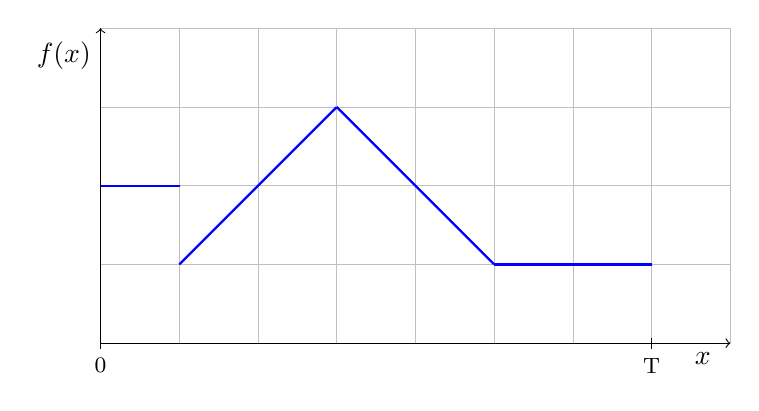
\begin{tikzpicture}[xscale=1, yscale=1]
	
	% Gitternetzlinien
	\draw[xstep=1cm, ystep=1cm, very thin, color=lightgray] (0,4) grid (8,0);
	% x-Achse
	\draw[->] (0,0) -- (8,0) node[below,xshift=-1em] {$x$}; 
	%Zahlen auf x-Achse
	%\foreach \x in {-3,...,-1}
	%\draw[shift={(\x,0)},color=black] (0pt,2pt) -- (0pt,-2pt) node[below] {\footnotesize $\x$};
	%\foreach \x in {1,...,3}
	%\draw[shift={(\x,0)},color=black] (0pt,2pt) -- (0pt,-2pt) node[below] {\footnotesize $\x$};
	% y-Achse 
	\draw[->] (0,0) -- (0,4) node[left,yshift=-1em] {$f(x)$};%node[above left]
	%Zahlen auf y-Achse
	%\foreach \y in {-1,...,-1}
	%\draw[shift={(0,\y)},color=black] (2pt,0pt) -- (-2pt,0pt) node[left] {\footnotesize $\y$};
	%\foreach \y in {1,...,3}
	%\draw[shift={(0,\y)},color=black] (2pt,0pt) -- (-2pt,0pt) node[left] {\footnotesize $\y$};
	%Ursprung
	
	\draw[shift={(7,0)},color=black] (0pt,2pt) -- (0pt,-2pt) node[below] {\footnotesize $\mathrm{T}$};
	\draw[shift={(0,0)},color=black] (0pt,2pt) -- (0pt,-2pt) node[below] {\footnotesize $\mathrm{0}$};
	\draw[thick,color=blue] plot[samples=200, domain=0:1] 
	(\x,{2});
	\draw[thick,color=blue] plot[samples=200, domain=1:3] 
	(\x,{\x});
	
	\draw[thick,color=blue] plot[samples=200, domain=3:5] 
	(\x,{-\x+6});
	\draw[thick,color=blue] plot[samples=200, domain=5:7] 
	(\x,{1});
	\end{tikzpicture}\\	
	
\end{center}
Dann gilt (ohne Beweis):\\
\begin{align*}
&f(x)=\phi_n(x)+\mathrm{R}_n(x)=\frac{a_0}{2}+\sum\limits_{k=1}^{n}a_k\cos(k\omega x)+b_k\sin(k\omega x)+\mathrm{R}_n(x)\\
&\mathrm{R}_n(x) = \;\;\text{Fehler }\\
&a_k, b_k \;=\;\;\text{Fourierkoeffizienten }\\
\end{align*}
Die Funktion: $ \mathrm{R}_n(x)=f(x) -\phi_n(x)$ erfüllt das Folgende:\\
\begin{align*}
\frac{2}{\mathrm{T}}\int\limits_{0}^{\mathrm{T}} \big(\mathrm{R}_n(x)\big)^2 \mathrm{d}x&=\frac{2}{\mathrm{T}}\int\limits_{0}^{\mathrm{T}} \bigg(f(x) -\phi_n(x)\bigg)^2 \mathrm{d}x\\
&\;\;\cdots\text{nach Umformung ergibt sich dann: }\\
&=\frac{2}{T}\int\limits_{0}^{\mathrm{T}} f^2(x)\mathrm{d}x-\bigg(\frac{a_0^2}{2}+\sum\limits_{k=1}^{n}(a^2_k+b^2_k)\bigg)\\
&\Leftrightarrow \;\;\text{für $ n\mapsto \infty  $ konvergiert dies gegen 0 und wird zur Pasevalschen Gleichung}\\
\frac{2}{T}\int\limits_{0}^{\mathrm{T}} f^2(x)\mathrm{d}x&=\bigg(\frac{a_0^2}{2}+\sum\limits_{k=1}^{\infty}(a^2_k+b^2_k)\bigg)\\
\end{align*}
Daraus folgt, dass der Fehler im quatratischen Mittel gegen 0 konvergiert.\\
\\
Die Parcevalsche Gleichung lautet:\\
\begin{center}
	\boxed{\frac{2}{T}\int\limits_{0}^{\mathrm{T}} f^2(x)\mathrm{d}x=\bigg(\frac{a_0}{2}^2+\sum\limits_{k=1}^{\infty}(a^2_k+b^2_k)\bigg)}
\end{center}
Ist $ f $ stetig in $ x $, so gilt:\\
\begin{align*}
\lim\limits_ {n\to\infty}\phi(x)=f(x)\Leftrightarrow\lim\limits_ {n\to\infty}\mathrm{R}(x)=0
\end{align*}
\newpage
\noindent
\subsubsection{ Beispiel zur Fourierapproximation}
\href{https://youtu.be/JnXjrvjlXg0}{Video 05}\\
Gegeben ist die $ 2\pi- $periodische Funktion $ f(x)=x $ für $ 0\leq x\leq 2\pi $.\\
Berechne das n-te Fourierpolynom.\\
\\
Wie sieht die Funktion aus ?\\
	\begin{center}
	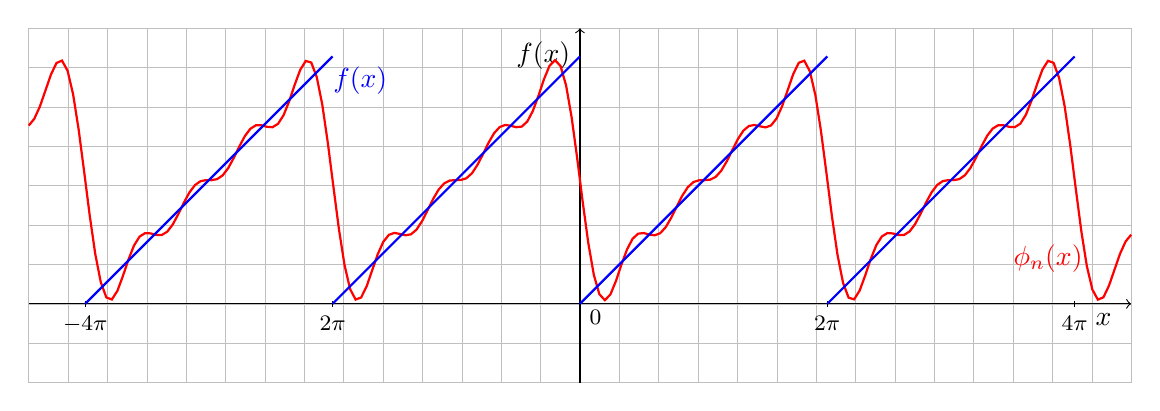
\begin{tikzpicture}[xscale=0.5, yscale=0.5]
	
	% Gitternetzlinien
	\draw[xstep=1cm, ystep=1cm, very thin, color=lightgray] (-14,7) grid (14,-2);
	% x-Achse
	\draw[->] (-14,0) -- (14,0) node[below,xshift=-1em] {$x$}; 
	%Zahlen auf x-Achse
	%\foreach \x in {-3,...,-1}
	%\draw[shift={(\x,0)},color=black] (0pt,2pt) -- (0pt,-2pt) node[below] {\footnotesize $\x$};
	%\foreach \x in {1,...,3}
	%\draw[shift={(\x,0)},color=black] (0pt,2pt) -- (0pt,-2pt) node[below] {\footnotesize $\x$};
	% y-Achse 
	\draw[->] (0,-2) -- (0,7) node[left,yshift=-1em] {$f(x)$};%node[above left]
	%Zahlen auf y-Achse
	%\foreach \y in {-1,...,-1}
	%\draw[shift={(0,\y)},color=black] (2pt,0pt) -- (-2pt,0pt) node[left] {\footnotesize $\y$};
	%\foreach \y in {1,...,3}
	%\draw[shift={(0,\y)},color=black] (2pt,0pt) -- (-2pt,0pt) node[left] {\footnotesize $\y$};
	%Ursprung
	\draw[color=black] (0pt,-10pt) node[right] {\footnotesize $0$};
	
	
	\draw[shift={(6.28,0)},color=black] (0pt,2pt) -- (0pt,-2pt) node[below] {\footnotesize $\mathrm{2\pi}$};
	\draw[shift={(-2*pi,0)},color=black] (0pt,2pt) -- (0pt,-2pt) node[below] {\footnotesize $\mathrm{2\pi}$};
	
	\draw[shift={(-4*pi,0)},color=black] (0pt,2pt) -- (0pt,-2pt) node[below] {\footnotesize $\mathrm{-4\pi}$};
	\draw[shift={(4*pi,0)},color=black] (0pt,2pt) -- (0pt,-2pt) node[below] {\footnotesize $\mathrm{4\pi}$};
	\draw[thick,color=red] plot[samples=200, domain=-14:14] 
	(\x,{pi-2*(sin(\x r)+0.5*sin((2*\x )r)+0.33*sin((3*\x )r)+0.25*sin((4*\x )r)) }) node[below, xshift=-3em]{$\phi_n(x)$};
	
	\draw[thick,color=blue] plot[samples=200, domain=0:2*pi] 
	(\x,{\x } );
	\draw[thick,color=blue] plot[samples=200, domain=2*pi:4*pi] 
	(\x,{\x-2*pi } );
	\draw[thick,color=blue] plot[samples=200, domain=-2*pi:0] 
	(\x,{\x +2*pi} );
	\draw[thick,color=blue] plot[samples=200, domain=-4*pi:-2*pi] 
	(\x,{\x +4*pi} ) node[below, xshift=1em]{$f(x)$};
	\end{tikzpicture}\\	
\end{center}
Berechnung der Koeffizienten $ a_0, a_k, b_k $ vom n-ten Fourierpolynoms:\\
\begin{align*}
\phi_n(x)=\frac{a_0}{2}+\sum\limits_{k=1}^{n}\big(a_k\cos(k\omega x)+b_k\sin(k\omega x)\big)
\end{align*}
Eine Periode ist zwischen 0 und $ 2\pi $ daraus folgt:\\
\begin{align*}
2\pi=\mathrm{T}=\frac{2\pi}{\omega}\Rightarrow \omega=1
\end{align*}
$ \bullet $\; Bestimmung von $ a_0 $:\\
\begin{align*}
a_0=\frac{2}{\mathrm{T}}\int\limits_{0}^{\mathrm{T}} f(x)\mathrm{d}x&=\frac{2}{2\pi}\int\limits_{0}^{2\pi} x\mathrm{d}x=\frac{1}{\pi}\bigg[\frac{x^2}{2}\bigg]^{2\pi}_0\\
&=\frac{1}{\pi}\bigg(\frac{(2\pi)^2}{2}-\frac{0^2}{2}\bigg)=\frac{1}{\pi}\frac{(2\pi)^2}{2}=\frac{4\pi^2}{\pi2}=2\pi\\
a_0&=2\pi
\end{align*}
\href{https://youtu.be/i4RYWjoYFAA}{Video 06}\\
$ \bullet $\;Bestimmung von $ a_k $:
\begin{align*}
a_k=\frac{2}{\mathrm{T}}\int\limits_{0}^{\mathrm{T}} f(x)\cdot \cos(kx)\mathrm{d}x=\frac{2}{2\pi}\int\limits_{0}^{2\pi} x\cdot \cos(kx)\mathrm{d}x
\end{align*}
\begin{quote}
	NR.: partielle Integration von: $ \int\limits_{}^{} x\cdot +\cos(x)\mathrm{d}x $\\
	\begin{align*}
	&u(x)=x\;\;\;\;\;\;\;\;\;\;\Rightarrow u'(x)=1\\
	&v'(x)=\cos(kx)\Rightarrow v(x)=\frac{1}{k}\sin(kx)\\
	&\int\limits_{}^{}x\cdot \cos(kx)\mathrm{d}x=\frac{1}{k}x\cdot \sin(kx)-\int\limits_{}^{} \frac{1}{k}\sin(kx)\mathrm{d}x\\
	&\int\limits_{}^{}x\cdot \cos(kx)\mathrm{d}x=\frac{1}{k}x\cdot \sin(kx)+\frac{1}{k^2}\cos(kx)
	\end{align*}
\end{quote}
\begin{align*}
a_k&=\frac{1}{\pi}\int\limits_{0}^{\pi} x\cdot \cos(kx)\mathrm{d}x\\
&=\frac{1}{\pi}\bigg( \frac{1}{k}\bigg[x\cdot \sin(kx)\bigg]^{2\pi}_0+\frac{1}{k^2}\bigg[\cos(kx)\bigg]^{2\pi}_0\bigg)\\
&=\frac{1}{\pi}\bigg(\frac{1}{k}(2\pi\cdot 0-0\cdot 0)+\frac{1}{k^2}(1-1)\bigg)=0\\
a_k&=0\;\;\text{für }\;\;k>0
\end{align*}
\href{https://youtu.be/Awz46xIlbyc}{Video 07}\\
$ \bullet $\;Bestimmung von $ b_k $:\\
\begin{align*}
b_k=\frac{2}{\mathrm{T}}\int\limits_{0}^{\mathrm{T}} f(x)\cdot \sin(kx)\mathrm{d}x=\frac{2}{2\pi}\int\limits_{0}^{2\pi} x\cdot \sin(kx)\mathrm{d}x
\end{align*}
\begin{quote}
	N.R.: partielle Integration von: $ \int\limits_{}^{} x\cdot \sin(x)\mathrm{d}x $\\
	\begin{align*}
	&u(x)=x\;\;\;\;\;\;\;\;\;\;\Rightarrow u'(x)=1\\
	&v'(x)=\sin(kx)\Rightarrow v(x)=-\frac{1}{k}\cos(kx)\\
	&\int\limits_{}^{}x\cdot \sin(kx)\mathrm{d}x=-\frac{1}{k}x\cdot \cos(kx)-\int\limits_{}^{} -\frac{1}{k}\cos(kx)\mathrm{d}x\\
	&\int\limits_{}^{}x\cdot \sin(kx)\mathrm{d}x=-\frac{1}{k}x\cdot \cos(kx)+\frac{1}{k^2}\sin(kx)
	\end{align*}
\end{quote}
\begin{align*}
b_k&=\frac{1}{\pi}\int\limits_{0}^{2\pi} x\cdot \sin(kx)\mathrm{d}x\\
&=\frac{1}{\pi}\bigg(-\frac{1}{k}\bigg[x\cdot \cos(kx)\bigg]^{2\pi}_0+\frac{1}{k^2}\bigg[\sin(kx)\bigg]^{2\pi}_0\bigg)\\
&=\frac{1}{\pi}\bigg(-\frac{1}{k}(2\pi-0)+\frac{1}{k^2}(0-0)\bigg)=\frac{-2\pi}{\pi k}\\
b_k&=-\frac{2}{k}
\end{align*}
Bemerkung:\\ Das Integral: $ \int\limits_{0}^{2\pi} \cos(x)\mathrm{d}x $ muß ja Null sein, weil die Summe der Flächen unter den Graphen Null über eine Periode ergeben muß. Analog auch der Sinus. \\
\\
\\
\\
\\
\\
\\
	\begin{center}
		Summe der Flächen ist Null.\\
	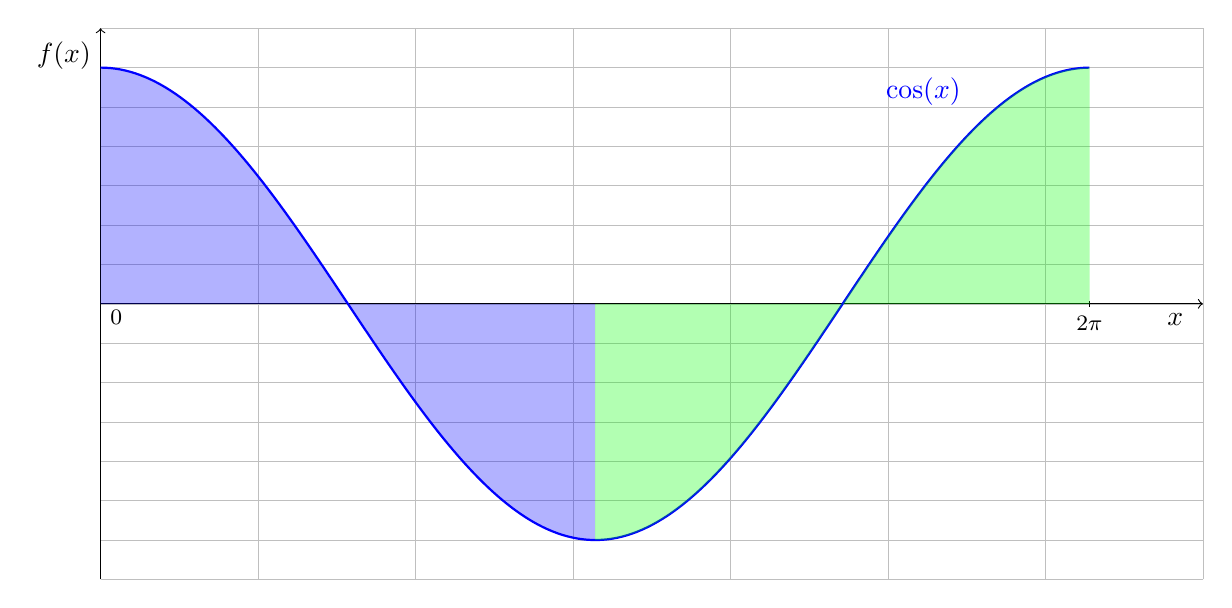
\begin{tikzpicture}[xscale=2, yscale=0.5]
	
	% Gitternetzlinien
	\draw[xstep=1cm, ystep=1cm, very thin, color=lightgray] (0,7) grid (7,-7);
	% x-Achse
	\draw[->] (0,0) -- (7,0) node[below,xshift=-1em] {$x$}; 
	%Zahlen auf x-Achse
	%\foreach \x in {-3,...,-1}
	%\draw[shift={(\x,0)},color=black] (0pt,2pt) -- (0pt,-2pt) node[below] {\footnotesize $\x$};
	%\foreach \x in {1,...,3}
	%\draw[shift={(\x,0)},color=black] (0pt,2pt) -- (0pt,-2pt) node[below] {\footnotesize $\x$};
	% y-Achse 
	\draw[->] (0,-7) -- (0,7) node[left,yshift=-1em] {$f(x)$};%node[above left]
	%Zahlen auf y-Achse
	%\foreach \y in {-1,...,-1}
	%\draw[shift={(0,\y)},color=black] (2pt,0pt) -- (-2pt,0pt) node[left] {\footnotesize $\y$};
	%\foreach \y in {1,...,3}
	%\draw[shift={(0,\y)},color=black] (2pt,0pt) -- (-2pt,0pt) node[left] {\footnotesize $\y$};
	%Ursprung
	\draw[color=black] (0pt,-10pt) node[right] {\footnotesize $0$};
	
	
	\draw[shift={(6.28,0)},color=black] (0pt,2pt) -- (0pt,-2pt) node[below] {\footnotesize $\mathrm{2\pi}$};
%	\draw[shift={(-2*pi,0)},color=black] (0pt,2pt) -- (0pt,-2pt) node[below] {\footnotesize $\mathrm{2\pi}$};
	
%	\draw[shift={(-4*pi,0)},color=black] (0pt,2pt) -- (0pt,-2pt) node[below] {\footnotesize $\mathrm{-4\pi}$};
%	\draw[shift={(4*pi,0)},color=black] (0pt,2pt) -- (0pt,-2pt) node[below] {\footnotesize $\mathrm{4\pi}$};
	\draw[thick,color=blue] plot[samples=200, domain=0:6.28] 
	(\x,{6*(cos(\x r)) }) node[below, xshift=-6em]{$\cos(x)$};
	\fill[color =blue,fill opacity=0.3] plot[domain=0:1.57] (\x,{6*(cos(\x r))})% 
	-- plot[domain=1.57:0] (\x,{0});% 
		\fill[color =blue,fill opacity=0.3] plot[domain=1.57:3.14] (\x,{6*(cos(\x r))})% 
	-- plot[domain=3.14:1.57] (\x,{0});% 
		\fill[color =green,fill opacity=0.3] plot[domain=3.14:4.71] (\x,{6*(cos(\x r))})% 
	-- plot[domain=4.71:3.14] (\x,{0});% 
		\fill[color =green,fill opacity=0.3] plot[domain=4.71:6.28] (\x,{6*(cos(\x r))})% 
	-- plot[domain=6.28:4.71] (\x,{0});% 

	\end{tikzpicture}\\	
\end{center}
Fazit: \\
Für das Fourierplynom mit $ \omega =1,\; a_0=2\pi,\; a_k=0 $ und $ b_k=-\frac{2}{k} $ gilt dann:\\
\begin{align*}
\phi_n(x)&=\frac{a_0}{2}+\sum\limits_{k=1}^{n}\big(a_k\cos(k\omega x)+b_k\sin(k\omega x)\big)\\
&=\pi+\sum\limits_{k=1}^{n}-\frac{2}{k}\sin(kx)\\
\phi_n(x)&=\pi-\sum\limits_{k=1}^{n}\frac{2}{k}\sin(kx)\\
\end{align*}
\href{https://youtu.be/7VbdjMYAqLM}{Video 08}\\
\underline {I. Konvergenzbetrachtung an der Stelle: $ x=\frac{\pi}{2} $.}\\
Ist $ f $ in $ x $ stetig, dann gilt:\\
\begin{align*}
\lim\limits_ {n\to\infty}\phi_n(x)=f(x)
\end{align*}
Für $ x=\frac{\pi}{2} $ und ist die Funktion: $ f(x)=x $ stetig, dann gilt:\\
\begin{align*}
&f(\genfrac{}{}{}{2}{\pi}{2 })=\lim\limits_ {n\to\infty}\phi_n(\genfrac{}{}{}{2}{\pi }{2 })\\
&\Rightarrow\\
&\frac{\pi}{2}=\lim\limits_ {n\to\infty}\bigg(\pi-\sum\limits_{k=1}^{n}\frac{2}{k}\sin(k\genfrac{}{}{}{2}{\pi }{2 })\bigg)\\
&\frac{\pi}{2}=\pi-\sum\limits_{k}^{\infty}\frac{2}{k}\cdot \sin(k\genfrac{}{}{}{2}{\pi }{2 })
\end{align*}
NR.:\\
Für $ \sum\limits_{k=1}^{\infty} \sin(k\genfrac{}{}{}{2}{\pi }{2})$ gilt:\\
	\begin{center}

	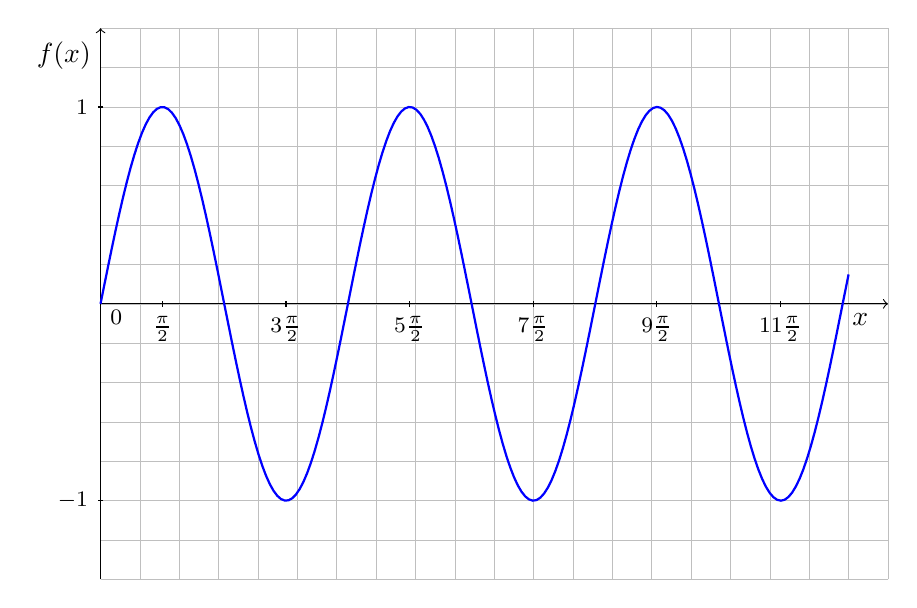
\begin{tikzpicture}[xscale=0.5, yscale=0.5]
	
	% Gitternetzlinien
	\draw[xstep=1cm, ystep=1cm, very thin, color=lightgray] (0,7) grid (20,-7);
	% x-Achse
	\draw[->] (0,0) -- (20,0) node[below,xshift=-1em] {$x$}; 
	%Zahlen auf x-Achse
	%\foreach \x in {-3,...,-1}
	%\draw[shift={(\x,0)},color=black] (0pt,2pt) -- (0pt,-2pt) node[below] {\footnotesize $\x$};
	%\foreach \x in {1,...,3}
	%\draw[shift={(\x,0)},color=black] (0pt,2pt) -- (0pt,-2pt) node[below] {\footnotesize $\x$};
	% y-Achse 
	\draw[->] (0,-7) -- (0,7) node[left,yshift=-1em] {$f(x)$};%node[above left]
	%Zahlen auf y-Achse
	%\foreach \y in {-1,...,-1}
	%\draw[shift={(0,\y)},color=black] (2pt,0pt) -- (-2pt,0pt) node[left] {\footnotesize $\y$};
	%\foreach \y in {1,...,3}
	%\draw[shift={(0,\y)},color=black] (2pt,0pt) -- (-2pt,0pt) node[left] {\footnotesize $\y$};
	%Ursprung
	\draw[shift={(0,5)},color=black] (2pt,0pt) -- (-2pt,0pt) node[left] {\footnotesize $1$};
	\draw[shift={(0,-5)},color=black] (2pt,0pt) -- (-2pt,0pt) node[left] {\footnotesize $-1$};
	\draw[color=black] (0pt,-10pt) node[right] {\footnotesize $0$};
	\draw[shift={(1.57,0)},color=black] (0pt,2pt) -- (0pt,-2pt) node[below] {\footnotesize $\frac{\pi}{2}$};
	\draw[shift={(3*1.57,0)},color=black] (0pt,2pt) -- (0pt,-2pt) node[below] {\footnotesize $3\frac{\pi}{2}$};

	\draw[shift={(5*1.57,0)},color=black] (0pt,2pt) -- (0pt,-2pt) node[below] {\footnotesize $5\frac{\pi}{2}$};
		\draw[shift={(7*1.57,0)},color=black] (0pt,2pt) -- (0pt,-2pt) node[below] {\footnotesize $7\frac{\pi}{2}$};
			\draw[shift={(9*1.57,0)},color=black] (0pt,2pt) -- (0pt,-2pt) node[below] {\footnotesize $9\frac{\pi}{2}$};
				\draw[shift={(11*1.57,0)},color=black] (0pt,2pt) -- (0pt,-2pt) node[below] {\footnotesize $11\frac{\pi}{2}$};
	%	\draw[shift={(-2*pi,0)},color=black] (0pt,2pt) -- (0pt,-2pt) node[below] {\footnotesize $\mathrm{2\pi}$};
	
	%	\draw[shift={(-4*pi,0)},color=black] (0pt,2pt) -- (0pt,-2pt) node[below] {\footnotesize $\mathrm{-4\pi}$};
	%	\draw[shift={(4*pi,0)},color=black] (0pt,2pt) -- (0pt,-2pt) node[below] {\footnotesize $\mathrm{4\pi}$};
	\draw[thick,color=blue] plot[samples=200, domain=0:19] 
	(\x,{5*(sin(\x r)) });

	
	\end{tikzpicture}\\	
\end{center}
Es gilt für k gerade:\\
\begin{align*}
&k=2=\sin(2\genfrac{}{}{}{2}{\pi }{2 })=0\\
&k=4=\sin(4\genfrac{}{}{}{2}{\pi }{2 })=0\\
&k=6=\sin(6\genfrac{}{}{}{2}{\pi }{2 })=0\\
&\colon
\end{align*}
Es gilt für k ungerade:\\
\begin{align*}
&k=1\Rightarrow\sin(1\genfrac{}{}{}{2}{\pi }{2 })=1\\
&k=3\Rightarrow\sin(3\genfrac{}{}{}{2}{\pi }{2 })=-1\\
&k=5\Rightarrow\sin(5\genfrac{}{}{}{2}{\pi }{2 })=1\\
&k=7\Rightarrow\sin(7\genfrac{}{}{}{2}{\pi }{2 })=-1\\
&\colon
\end{align*}
Ebenso gilt :\\
\begin{align*}
&\sum\limits_{n=1}^{\infty}\big(-1)^{n-1}=\sum\limits_{k=1}^{\infty}\sin(k\genfrac{}{}{}{2}{\pi }{2 })\;\;\text{für $ k $ ungerade } \\
&n=1\Rightarrow 1\\
&n=2\Rightarrow -1\\
&n=3\Rightarrow 1\\
&\colon
\end{align*}

\newpage
Also gilt dann für: $ \frac{\pi}{2}=\pi-\sum\limits_{k}^{\infty}\frac{2}{k}\cdot \sin(k\genfrac{}{}{}{2}{\pi }{2 }) $:\\
\begin{align*}
&\frac{\pi}{2}=\pi-\sum\limits_{n=1}^{\infty}\bigg(\frac{2}{(2n-1)}\big(-1\big)^{n-1}\bigg)\\
&\Leftrightarrow\\
&\sum\limits_{n=1}^{\infty}\bigg(\frac{2}{(2n-1)}\big(-1\big)^{n-1}\bigg)=\frac{\pi}{2}\\
&\Leftrightarrow\\
&\sum\limits_{n=1}^{\infty}\bigg(\frac{1}{(2n-1)}\big(-1\big)^{n-1}\bigg)=\frac{\pi}{4}\\
\end{align*}
Diese Reihe ist die Leibnitz-Reihe.\\
\href{https://youtu.be/81emk4QNvwc}{Video 09}\\
\underline{II. Konvergenzverhalten mit Pasevalscher Gleichung:}\\
\\
Pasevalsche Gleichung:\\
\begin{align*}
\frac{2}{T}\int\limits_{0}^{\mathrm{T}} f^2(x)\mathrm{d}x&=\bigg(\frac{a_0^2}{2}+\sum\limits_{k=1}^{\infty}(a^2_k+b^2_k)\bigg)\\
\end{align*}
Nun gilt für $ T=2\pi, f(x)=x, a_0=2\pi, a_k=0, b_k=-\frac{2}{k} $:\\
\begin{align*}
\frac{2}{2\pi}\int\limits_{0}^{2\pi} x^2\mathrm{d}x=\frac{4\pi^2}{2}+\sum\limits_{k=1}^{\infty}\frac{4}{k^2}
\end{align*}
Integral von $\frac{1}{\pi}\int\limits_{0}^{2\pi} x^2\mathrm{d}x  $ berechnen:\\
\begin{align*}
\frac{1}{\pi}\int\limits_{0}^{2\pi} x^2\mathrm{d}x&=\frac{1}{\pi}\bigg[\frac{x^3}{3}\bigg]^{2\pi}_0=\frac{1}{\pi}\cdot\frac{8\pi^3}{3}=\frac{8\pi^2}{3}
\end{align*}
Dann erhält man:\\
\begin{align*}
&\frac{8\pi^2}{3}=2\pi^2+\sum\limits_{k=1}^{\infty}\frac{4}{k^2}\\
&\Leftrightarrow \frac{8\pi^2}{3}-2\pi^2=\sum\limits_{k=1}^{\infty}\frac{4}{k^2}\\
&\,\;\;\;\;\;\;\;\;\;\;\;\;\;\;\;\frac{2}{3}\pi^2=\sum\limits_{k=1}^{\infty}\frac{4}{k^2}\\
&\Leftrightarrow\\
&\,\;\;\;\;\;\;\;\;\;\;\;\;\;\;\;\frac{1}{3}\pi^2=\sum\limits_{k=1}^{\infty}\frac{2}{k^2}
\end{align*}
\subsubsection{Aufgabe zur Fourierapproximation }
\href{https://youtu.be/USTvFINpj6I}{Video 10}\\
Gegeben ist die $\pi$-periodische Funktion $ f(x)=\big(x-\frac{\pi}{2}\big)^2 $ für $ 0\leq x \leq\pi $.\\
(i) \;\;Skizziere den Graph von $ f $.\\
(ii)\; Berechne das n-te Fourierpolynom von $ f $.\\
(iii) Zeige:\\
\begin{align*}
\sum\limits_{n=1}^{\infty}\frac{(-1)^{n-1}}{n^2}=\frac{\pi^2}{12}
\end{align*}
zu (i): Skizze von der $\pi$ -periodischen Funktion: $ f(x)=\big(x-\frac{\pi}{2}\big)^2$ für $ 0\leq x \leq\pi $\\
	\begin{center}
	
	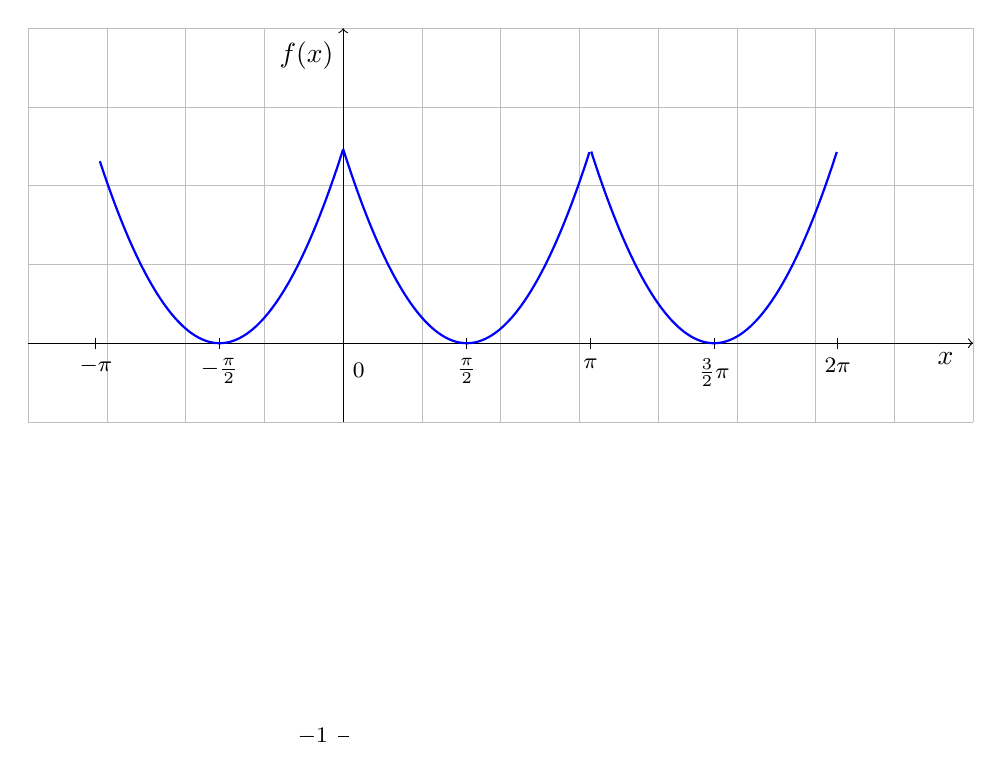
\begin{tikzpicture}[xscale=1, yscale=1]
	% Gitternetzlinien
	\draw[xstep=1cm, ystep=1cm, very thin, color=lightgray] (-4,4) grid (8,-1);
	% x-Achse
	\draw[->] (-4,0) -- (8,0) node[below,xshift=-1em] {$x$}; 
	%Zahlen auf x-Achse
	%\foreach \x in {-3,...,-1}
	%\draw[shift={(\x,0)},color=black] (0pt,2pt) -- (0pt,-2pt) node[below] {\footnotesize $\x$};
	%\foreach \x in {1,...,3}
	%\draw[shift={(\x,0)},color=black] (0pt,2pt) -- (0pt,-2pt) node[below] {\footnotesize $\x$};
	% y-Achse 
	\draw[->] (0,-1) -- (0,4) node[left,yshift=-1em] {$f(x)$};%node[above left]
	%Zahlen auf y-Achse
	%\foreach \y in {-1,...,-1}
	%\draw[shift={(0,\y)},color=black] (2pt,0pt) -- (-2pt,0pt) node[left] {\footnotesize $\y$};
	%\foreach \y in {1,...,3}
	%\draw[shift={(0,\y)},color=black] (2pt,0pt) -- (-2pt,0pt) node[left] {\footnotesize $\y$};
	%Ursprung
	%\draw[shift={(0,5)},color=black] (2pt,0pt) -- (-2pt,0pt) node[left] {\footnotesize $1$};
	\draw[shift={(0,-5)},color=black] (2pt,0pt) -- (-2pt,0pt) node[left] {\footnotesize $-1$};
	\draw[color=black] (0pt,-10pt) node[right] {\footnotesize $0$};
	\draw[shift={(1.57,0)},color=black] (0pt,2pt) -- (0pt,-2pt) node[below] {\footnotesize $\frac{\pi}{2}$};
	\draw[shift={(3.14,0)},color=black] (0pt,2pt) -- (0pt,-2pt) node[below] {\footnotesize $\pi$};
	
	%\draw[shift={(5*1.57,0)},color=black] (0pt,2pt) -- (0pt,-2pt) node[below] {\footnotesize $5\frac{\pi}{2}$};
	\draw[shift={(6.28,0)},color=black] (0pt,2pt) -- (0pt,-2pt) node[below] {\footnotesize $2\pi$};
	\draw[shift={(-3.14,0)},color=black] (0pt,2pt) -- (0pt,-2pt) node[below] {\footnotesize $-\pi$};
	\draw[shift={(4.71,0)},color=black] (0pt,2pt) -- (0pt,-2pt) node[below] {\footnotesize $\frac{3}{2}\pi$};
		\draw[shift={(-1.57,0)},color=black] (0pt,2pt) -- (0pt,-2pt) node[below] {\footnotesize $-\frac{\pi}{2}$};
	%\draw[shift={(11*1.57,0)},color=black] (0pt,2pt) -- (0pt,-2pt) node[below] {\footnotesize $11\frac{\pi}{2}$};
	%	\draw[shift={(-2*pi,0)},color=black] (0pt,2pt) -- (0pt,-2pt) node[below] {\footnotesize $\mathrm{2\pi}$};
	
	%	\draw[shift={(-4*pi,0)},color=black] (0pt,2pt) -- (0pt,-2pt) node[below] {\footnotesize $\mathrm{-4\pi}$};
	%	\draw[shift={(4*pi,0)},color=black] (0pt,2pt) -- (0pt,-2pt) node[below] {\footnotesize $\mathrm{4\pi}$};
	\draw[thick,color=blue] plot[samples=200, domain=0:3.13] 
	(\x,{(\x-1.57))^2 }); 
		\draw[thick,color=blue] plot[samples=200, domain=3.15:6.27] 
	(\x,{(\x-4.71))^2 }); 
		\draw[thick,color=blue] plot[samples=200, domain=-3.09:0] 
	(\x,{(\x+1.57))^2 }); 
	\end{tikzpicture}\\	
\end{center}
zu (ii): Berechnung von $ \phi_n(x)=\frac{a_0}{2}+\sum\limits_{k=1}^{n}\big(a_k\cos(k\omega x)+b_k\sin(k\omega x)\big) $\\
\begin{quote}
	Berechnen von $ \omega $:\\
	\begin{align*}
	&\mathrm{T}=\pi\\
	&\mathrm{T}=\frac{2\pi}{\omega}\overset{!}{=}\pi\Rightarrow \omega=2
	\end{align*}
	\newpage
	$\bullet$ \;\; Bestimmung von $a_0$:\\
	\begin{align*}
	a_0&=\frac{2}{\mathrm{T}}\int\limits_{0}^{\mathrm{T}} f(x)\mathrm{d}x\\
	&=\frac{2}{\pi}\int\limits_{0}^{\pi} \bigg(x-\frac{\pi}{2}\bigg)^2\mathrm{d}x\\
	&=\frac{2}{\pi}\Bigg[\frac{1}{3}\bigg(x-\frac{\pi}{2}\bigg)^3\Bigg]^\pi_0=\frac{2}{3\pi}\Bigg[\bigg(x-\frac{\pi}{2}\bigg)^3\Bigg]^\pi_0\\
	&=\frac{2}{3\pi}\Bigg[\bigg(0-\frac{\pi}{2}\bigg)^3-\bigg(\pi-\frac{\pi}{2}\bigg)^3\Bigg]\\
		&=\frac{2}{3\pi}\Bigg[\bigg(\frac{\pi}{2}\bigg)^3+\bigg(\frac{\pi}{2}\bigg)^3\Bigg]=\frac{2}{3\pi}\bigg(2\bigg(\frac{\pi}{2}\bigg)^3\bigg)=\frac{\pi^2}{3\cdot 2}\\
		a_0&=\frac{\pi^2}{6}
	\end{align*}
\href{https://youtu.be/BAyYyKjnVSE}{Video 11}\\
$\bullet$ \;\; Bestimmung von $a_k$:\\
\begin{align*}
a_k=\frac{2}{\mathrm{T}}\int\limits_{0}^{\mathrm{T}} f(x)\cos(k\omega x)\mathrm{d}x=\frac{2}{\pi}\int\limits_{0}^{\pi}\bigg(x-\frac{\pi}{2}\bigg)^2\cos(k2x)\mathrm{d}x \\
\end{align*}
NR.: partielle Integration von: $\int\limits_{}^{}\big(x-\frac{\pi}{2}\big)^2\cos(k2x)\mathrm{d}x  $\\
\begin{align*}
&u(x)=\bigg(x-\frac{\pi}{2}\bigg)^2\Rightarrow u'(x)=2\bigg(x-\frac{\pi}{2}\bigg)\\
&v'(x)=\cos(k2x)\;\;\Rightarrow v(x)=\frac{1}{2k}\sin(k2x)
\end{align*}
\begin{align*}
\int\limits_{}^{}\bigg(x-\frac{\pi}{2}\bigg)^2\cos(k2x)\mathrm{d}x& =\bigg(x-\frac{\pi}{2}\bigg)^2\frac{1}{2k}\sin(k2x)-\int\limits_{}^{} 2\bigg(x-\frac{\pi}{2}\bigg)\frac{1}{2k}\sin(k2x)\mathrm{d}x\\
&=\bigg(x-\frac{\pi}{2}\bigg)^2\frac{1}{2k}\sin(k2x)-\frac{1}{k}\int\limits_{}^{} \bigg(x-\frac{\pi}{2}\bigg)\sin(k2x)\mathrm{d}x
\end{align*}
Für das bestimmte Integral von $ \int\limits_{0}^{\pi}  $ gilt:\\
\begin{align*}
\int\limits_{0}^{\pi}\bigg(x-\frac{\pi}{2}\bigg)^2\cos(k2x)\mathrm{d}x&=\bigg[\bigg(x-\frac{\pi}{2}\bigg)^2\frac{1}{2k}\sin(k2x)\bigg]^\pi_0-\int\limits_{0}^{\pi} \bigg(x-\frac{\pi}{2}\bigg)\sin(k2x)\mathrm{d}x \\
&=0-\int\limits_{0}^{\pi} \bigg(x-\frac{\pi}{2}\bigg)\sin(k2x)\mathrm{d}x \\
\end{align*}
Nochmalige partielle Integration von $\int\limits_{}^{} \big(x-\frac{\pi}{2}\big)\sin(k2x)\mathrm{d}x  $\\
\begin{align*}
&u(x)=x-\frac{\pi}{2}\;\;\;\;\Rightarrow u'(x)=1\\
&v'(x)=\sin(2kx)\Rightarrow v(x)=-\frac{1}{2k}\cos(2kx)
\end{align*}
\begin{align*}
\int\limits_{}^{} \bigg(x-\frac{\pi}{2}\bigg)\sin(k2x)\mathrm{d}x&=\bigg(x-\frac{\pi}{2}\bigg)\bigg(-\frac{1}{2k}\cos(2kx)\bigg)-\int\limits_{}^{}-\frac{1}{2k}\cos(2kx)\mathrm{d} x\\
&=\bigg(x-\frac{\pi}{2}\bigg)\bigg(-\frac{1}{2k}\cos(2kx)\bigg)+\frac{1}{2k}\int\limits_{}^{}\cos(2kx)\mathrm{d} x\\
\end{align*}
Für das bestimmte Integral von $ \int\limits_{o}^{\pi}  $ gilt, weil das Integral: $ \int\limits_{0}^{\pi}\cos(2kx) =0 $:\\
\begin{align*}
\int\limits_{0}^{\pi} \bigg(x-\frac{\pi}{2}\bigg)\sin(k2x)\mathrm{d}x=\bigg(x-\frac{\pi}{2}\bigg)\bigg(-\frac{1}{2k}\cos(2kx)\bigg)+0
\end{align*}
Nun ergibt sich das Integral von:$ \int\limits_{}^{}\big(x-\frac{\pi}{2}\big)^2\cos(k2x)\mathrm{d}x $:\\
\begin{align*}
\int\limits_{}^{}\bigg(x-\frac{\pi}{2}\bigg)^2\cos(k2x)\mathrm{d}x=-\frac{1}{k} \bigg(x-\frac{\pi}{2}\bigg)\bigg(-\frac{1}{2k}\cos(2kx)\bigg)=\frac{1}{k} \bigg(x-\frac{\pi}{2}\bigg)\bigg(\frac{1}{2k}\cos(2kx)\bigg)
\end{align*}
Nun ergibt sich für $ a_k $:\\
\begin{align*}
a_k&=\frac{2}{\pi}\int\limits_{0}^{\pi}\frac{1}{k} \bigg(x-\frac{\pi}{2}\bigg)^2\cos(k2x)\mathrm{d}x\\
&=\frac{2}{k\pi}\bigg[\bigg(x-\frac{\pi}{2}\bigg)\bigg(\frac{1}{2k}\cos(2kx)\bigg)\bigg]^\pi_0\\
&=\frac{1}{\pi k^2}\bigg[\bigg(x-\frac{\pi}{2}\bigg)\cos(2kx)\bigg]^\pi_0\\&=\frac{1}{\pi k^2}\bigg[\bigg(\pi-\frac{\pi}{2}\bigg)\cos(2k\pi)-\bigg(0-\frac{\pi}{2}\bigg)\cos(2k 0)\bigg]\\
&=\frac{1}{\pi k^2}\bigg(\frac{\pi}{2}+\frac{\pi}{2}\bigg)=\frac{1}{\pi k^2}\pi\\
a_k&=\frac{1}{k^2}
\end{align*}
\href{https://youtu.be/3sByNrjJVc0}{Video 12}\\
$\bullet$ \;\; Bestimmung von $b_k$:\\
\begin{align*}
b_k=\frac{1}{\mathrm{T}}\int\limits_{0}^{\mathrm{T}}f(x) \sin(k\omega x)\mathrm{d}x=\frac{2}{\pi}\int\limits_{0}^{\pi} \bigg(x-\frac{\pi}{2}\bigg)^2\sin(k2x)\mathrm{d}x
\end{align*}
NR.: partielle Integration von: $\int\limits_{}^{} \big(x-\frac{\pi}{2}\big)^2\sin(k2x)\mathrm{d}x  $\\
\begin{align*}
&u(x)=\bigg(x-\frac{\pi}{2}\bigg)^2\Rightarrow u'(x)=2\bigg(x-\frac{\pi}{2}\bigg)\\
&v'(x)=\sin(2kx)\Rightarrow v(x)\;=-\frac{1}{2k}\cos(2kx)
\end{align*}
\begin{align*}
\int\limits_{}^{} \bigg(x-\frac{\pi}{2}\bigg)^2\sin(k2x)\mathrm{d}x&=\bigg(x-\frac{\pi}{2}\bigg)^2\bigg(-\frac{1}{2k}\cos(2kx)\bigg)-\int\limits_{}^{} 2\bigg(x-\frac{\pi}{2}\bigg)\bigg(-\frac{1}{2k}\cos(2kx)\bigg)\mathrm{d}x\\
&=-\frac{1}{2k}\bigg(x-\frac{\pi}{2}\bigg)^2\bigg(\cos(2kx)\bigg)+\frac{1}{k}\int\limits_{}^{} \bigg(x-\frac{\pi}{2}\bigg)\bigg(\cos(2kx)\bigg)\mathrm{d}x
\end{align*}
Für das bestimmte Integral von $ \int\limits_{0}^{\pi}  $ gilt:\\
\begin{align*}
\int\limits_{0}^{\pi}\bigg(x-\frac{\pi}{2}\bigg)^2\sin(k2x)\mathrm{d}x&=-\frac{1}{2k}\bigg[\bigg(x-\frac{\pi}{2}\bigg)^2\bigg(\cos(2kx)\bigg)\bigg]^\pi_0+\frac{1}{k}\int\limits_{0}^{\pi} \bigg(x-\frac{\pi}{2}\bigg)\bigg(\cos(2kx)\bigg)\mathrm{d}x\\
&=\frac{1}{k}\bigg(\bigg(\frac{\pi}{2}\bigg)^2-\bigg(\frac{\pi}{2}\bigg)^2\bigg)+\frac{1}{k}\int\limits_{0}^{\pi} \bigg(x-\frac{\pi}{2}\bigg)\bigg(\cos(2kx)\bigg)\mathrm{d}x\\
&=0+\frac{1}{k}\int\limits_{0}^{\pi} \bigg(x-\frac{\pi}{2}\bigg)\bigg(\cos(2kx)\bigg)\mathrm{d}x\\
\end{align*}
Nochmalige partielle Integration von: $ \int\limits_{}^{} \big(x-\frac{\pi}{2}\big)\big(\cos(2kx)\big)\mathrm{d}x $
\begin{align*}
&u(x)=x-\frac{\pi}{2}\;\;\;\;\Rightarrow u'(x)=1\\
&v'(x)=\cos(2kx)\Rightarrow v(x)=\frac{1}{2k}\sin(2kx)
\end{align*}
\begin{align*}
\int\limits_{}^{} \bigg(x-\frac{\pi}{2}\bigg)\bigg(-\frac{1}{2k}\cos(2kx)\bigg)\mathrm{d}x=\bigg(x-\frac{\pi}{2}\bigg)\bigg(\frac{1}{2k}\sin(2kx)\bigg)-\int\limits_{}^{} \frac{1}{2k}\sin(2kx)\mathrm{d}x\\
\end{align*}
Für das bestimmte Integral: $ \int\limits_{0}^{\pi}  $ gilt:\\
\begin{align*}
\int\limits_{0}^{\pi} \bigg(x-\frac{\pi}{2}\bigg)\bigg(-\frac{1}{2k}\cos(2kx)\bigg)\mathrm{d}x
&=\frac{1}{2k}\bigg[\bigg(x-\frac{\pi}{2}\bigg)\bigg(\sin(2kx)\bigg)\bigg]^\pi_0-\frac{1}{2k}\int\limits_{0}^{\pi} \sin(2kx)\mathrm{d}x\\
&=\bigg(\pi-\frac{\pi}{2}\bigg) \sin(2k\pi)-\bigg(0-\frac{\pi}{2}\bigg)\sin(2k 0)\bigg)-\frac{1}{2k}\cdot 0\\
&=0-0=0\\
&\Rightarrow \int\limits_{0}^{\pi} \bigg(x-\frac{\pi}{2}\bigg)\sin(k2x)\mathrm{d}x=0
\end{align*}
Nun ergibt sich für $ b_k $:\\
\begin{align*}
b_k=\frac{1}{\mathrm{T}}\int\limits_{0}^{\mathrm{T}}f(x) \sin(k\omega x)\mathrm{d}x&=\frac{2}{\pi}\int\limits_{0}^{\pi} \bigg(x-\frac{\pi}{2}\bigg)^2\sin(k2x)\mathrm{d}x\\
&=\frac{2}{\pi}\cdot 0
\end{align*}
\begin{align*}
b_k=\frac{1}{\pi}\cdot 0 =0
\end{align*}
Für das Fourierplynom mit $ \omega =2,\; a_0=\frac{\pi^2}{6}\pi, \;a_k=\frac{1}{k^2} $ und $ b_k=0 $ gilt dann:\\
\begin{align*}
&\phi(x)=\frac{a_0}{2}+\sum\limits_{k=1}^{n}(a_k\cos(k\omega x)+b_k\sin(k\omega x))\\
&\phi(x)=\frac{\pi^2}{12}+\sum\limits_{k=1}^{n}\frac{1}{k^2}\cos(k2x)
\end{align*}
\end{quote}
\href{https://youtu.be/IcA3p-nQn7Y}{Video 13}\\
zu (iii): Beweise:\\
\begin{align*}
\sum\limits_{n=1}^{\infty}\frac{(-1)^{n-1}}{n^2}=\frac{\pi^2}{12}
\end{align*}
\begin{quote}
 Da $ f(x) $ in $ \frac{\pi}{2} $ stetig ist gilt: $ f(\frac{\pi}{2})=\lim\limits_ {n\to\infty}\phi_n(\frac{\pi}{2})=\frac{\pi^2}{12}+\sum\limits_{n=1}^{\infty}\frac{1}{n}\cos(n2\cdot\frac{\pi}{2}) $.\\
Dann gilt:\\
\begin{align*}
 f(\genfrac{}{}{}{2}{\pi }{2 })=0=\lim\limits_ {n\to\infty}\bigg(\frac{\pi^2}{12}-\sum\limits_{n=1}^{\infty}\frac{1}{n^2}\cos(n\pi)\bigg)
\end{align*}
Für den $ \cos(n\pi) $ gilt:\\
\begin{align*}
&n=1\Rightarrow \cos(1\pi)=1\\
&n=2\Rightarrow \cos(2\pi)=-1\\
&n=3\Rightarrow \cos(3\pi)=1\\
&\colon\\
&\Rightarrow (-1)^{n-1}=\cos(n\pi)\;\;\text{für } n\geq 1
\end{align*}
Dann erhält man:\\
\begin{align*}
&f(\genfrac{}{}{}{2}{\pi }{2 })=0=\lim\limits_ {n\to\infty}\bigg(\frac{\pi}{12}-\sum\limits_{n=1}^{\infty}\frac{1}{n^2}(-1)^{n-1}\bigg)\\
&0=\frac{\pi}{12}-\sum\limits_{n=1}^{\infty}\frac{1}{n^2}(-1)^{n-1}\\
&\Leftrightarrow\\
&\sum\limits_{n=1}^{\infty}\frac{(-1)^{n-1}}{n^2}=\frac{\pi}{12}_{ _\Box}
\end{align*}
\end{quote}
\subsection{Komplexe Fourieranalysis/Komplexes Fourierpolynom}
\href{https://youtu.be/dZAkPwv7v28}{Video 14}\\
Sei $ f:\mathbb{R}\longmapsto \mathbb{R} $ eine $ \mathrm{T}=\frac{2\pi}{\omega} $ periodische monotone Funktion.\\
Wir wissen von  den kompexen Zahlen:\\
\begin{align*}
\mathrm{e}^{\mathrm{i}x}=\cos(x)+\mathrm{i}\sin(x)
\end{align*}
Dann gilt auch:\\
\begin{align*}
\cos(x)=\frac{\mathrm{e}^{\mathrm{ix}}+\mathrm{e}^{-\mathrm{i}x}}{2}\\
\sin(x)=\frac{\mathrm{e}^{\mathrm{ix}}-\mathrm{e}^{-\mathrm{i}x}}{2\mathrm{i}}\\
\end{align*}
Damit bekommt man durch Umformung von:\\
\begin{align*}
\phi_n(x)=\frac{a_0}{2}+\sum\limits_{k=1}^{n}\big(a_k\cos(k\omega x)+b_k\sin(k\omega x)\big)
\end{align*}
das komplexe Fourierpolynom:\\
\begin{align*}
\phi_n(x)&=\sum\limits_{k=-n}^{n}c_k\cdot \mathrm{e}^{\mathrm{i}kwx}\\
c_k&=\frac{1}{\mathrm{T}}\int\limits_{0}^{\mathrm{T}} f(x)\mathrm{e}^{-\mathrm{i}k\omega x}\mathrm{d}x
\end{align*}
\subsubsection{Beispiel zum komplexen Fourierpolynom Teil 1}
\href{https://youtu.be/PLrUWD6DO3g}{Video 15}\\
Betrachte die $ 2\pi $ -periodische Funktion $ f(x)=x $ für $ 0\leq x\leq\pi $ .\\
\\
Da $ \mathrm{T}=\frac{2\pi}{\omega} $ und $ \mathrm{T}=2\pi \Rightarrow \omega=1 $.\\
Zu berechnen:\\
\begin{align*}
\phi_n(x)&=\sum\limits_{k=-n}^{n}c_k\cdot \mathrm{e}^{\mathrm{i}kwx}\\
c_k&=\frac{1}{\mathrm{T}}\int\limits_{0}^{\mathrm{T}} f(x)\mathrm{e}^{-\mathrm{i}k\omega x}\mathrm{d}x
\end{align*}
Mit $f(x)=x,\; \mathrm{T}=2\pi $ und $ \omega=1 $ gilt:\\
\begin{align*}
c_k&=\frac{1}{2\pi}\int\limits_{0}^{\mathrm{2\pi}} x\cdot\mathrm{e}^{-\mathrm{i}k x}\mathrm{d}x
\end{align*}
NR.: partielle Integration von: $ \int\limits_{}^{} x\cdot \mathrm{e}^{-\mathrm{i}kx}\mathrm{d}x $\\
\begin{align*}
&u(x)=x\;\;\;\;\;\;\Rightarrow u'(x)=1\\
&v'(x)=\mathrm{e}^{-\mathrm{i}kx}\Rightarrow v(x)=-\frac{1}{\mathrm{i}k}\mathrm{e}^{-\mathrm{i}kx}
\end{align*}
\begin{align*}
\int\limits_{}^{}x\cdot \mathrm{e}^{-\mathrm{i}kx}\mathrm{d}x&=x\cdot-\frac{1}{\mathrm{i}k} \mathrm{e}^{-\mathrm{i}kx}+\frac{1}{\mathrm{i}k}\int\limits_{}^{}\mathrm{e}^{-\mathrm{i}kx} \mathrm{d}x\\
&=-\frac{1}{\mathrm{i}k}x\cdot \mathrm{e}^{-\mathrm{i}kx}+\frac{1}{\mathrm{i}k}\cdot\frac{1}{-\mathrm{i}k}\mathrm{e}^{-\mathrm{i}kx} \\
\end{align*}
Für das bestimmte Integral: $ \int\limits_{0}^{2\pi}  $ gilt:\\
\begin{align*}
\int\limits_{0}^{2\pi}x\cdot \mathrm{e}^{-\mathrm{i}kx}\mathrm{d}x&=-\frac{1}{\mathrm{i}k}\bigg[x\cdot \mathrm{e}^{-\mathrm{i}kx}\bigg]^{2\pi}_0+\frac{1}{k^2}\bigg[\mathrm{e}^{\mathrm{i}kx}\bigg]^{2\pi}_0\\
&=-\frac{1}{\mathrm{i}k}\big(2\pi\cdot\mathrm{e}^{\mathrm{i}2\pi}-0\cdot\mathrm{e}^{\mathrm{i}k0}\big)+\frac{1}{k^2}\big(\mathrm{e}^{\mathrm{i}k2\pi}-\mathrm{e}^{\mathrm{i}k0}\big)\\
\end{align*}
\begin{quote}
	NR.\\
	\begin{align*}
	\mathrm{e}^{\mathrm{i}k2\pi}=\big(\mathrm{e}^{\mathrm{i}\pi}\big)^{2k}=\big(-1\big)^{2k}=1
	\end{align*}
	oder:\\
	\begin{align*}
	\mathrm{e}^{\mathrm{i}k2\pi}=\cos(k2\pi)+\mathrm{i}\sin(k2\pi)=1-0=1
	\end{align*}
\end{quote}
So ergibt sich das bestimmte Integral:  $ \int\limits_{0}^{2\pi}  $ \\
\begin{align*}
\int\limits_{0}^{2\pi}x\cdot \mathrm{e}^{-\mathrm{i}kx}\mathrm{d}x&=-\frac{1}{\mathrm{i}k}(2\pi\cdot 1-0)+\frac{1}{k^2}(1-1)=-\frac{2\pi}{\mathrm{i}k}
\end{align*}
Dann gilt für $ c_k $:\\
\begin{align*}
c_k&=\frac{1}{2\pi}\int\limits_{0}^{\mathrm{2\pi}} x\cdot\mathrm{e}^{-\mathrm{i}k x}\mathrm{d}x\\
&=\frac{1}{2\pi}\cdot-\frac{2\pi}{\mathrm{i}k}=\frac{1}{-\mathrm{i}k}\\
\end{align*}
\begin{quote}
	Ebenso gilt:\\
	\begin{align*}
	\frac{-1}{\mathrm{i}}=\frac{\mathrm{i}\cdot (-1)}{\mathrm{i}\cdot \mathrm{i}}=\frac{\mathrm{i}\cdot (-1)}{\mathrm{i^2}}=\frac{-\mathrm{i}}{-1}=\mathrm{i}\Rightarrow \frac{-1}{\mathrm{i}k}=\mathrm{i}\frac{1}{k}
	\end{align*}
\end{quote}
Für $ k\neq 0 $ ergibt sich:\\
\begin{align*}
c_k=\mathrm{i}\frac{1}{k} \;\;\text{für } k\neq 0
\end{align*}
Für $ k= 0 $ ergibt sich dann: $ c_0 $\\
\begin{align*}
c_0&=\frac{1}{2\pi}\int\limits_{0}^{2\pi} x\cdot \mathrm{e}^{-\mathrm{i}kx}\mathrm{d}x\\
&=\frac{1}{2\pi}\int\limits_{0}^{2\pi} x\cdot \mathrm{e}^{0}\mathrm{d}x\\
&=\frac{1}{2\pi}\int\limits_{0}^{2\pi} x\mathrm{d}x=\frac{1}{2\pi}\bigg[\frac{x^2}{2}\bigg]^{2\pi}_0=\frac{1}{2\pi}\frac{(2\pi)^2}{2}=\frac{2\pi}{2}=\pi\\
\end{align*}
Fazit:\\
\begin{align*}
c_0&=\pi\\
c_k&=\frac{\mathrm{i}}{k}\;\;\text{für } k\neq 0\\
\phi_n(x)&=\pi+\sum\limits_{\substack{k=-n\\k\neq 0}}^{n}\frac{\mathrm{i}}{k}\mathrm{e}^{\mathrm{i}kx}
\end{align*}
\subsubsection{Beispiel zum komplexen Fourierpolynom Teil 2}
\href{https://youtu.be/Ln1HFYRNBsw}{Video 16}\\
Das komplexe Fourierpolynom in das reelle Fourierpolynom umwandeln.\\
\begin{align*}
\phi_n(x)&=\pi+\sum\limits_{\substack{k=-n\\k\neq 0}}^{n}\frac{\mathrm{i}}{k}\mathrm{e}^{\mathrm{i}kx}\;\;\arrowvert\text{\tiny Summe aufteilen }\\
&=\pi+\sum\limits_{k=-n}^{-1}\frac{\mathrm{i}}{k}\mathrm{e}^{\mathrm{i}kx}+\sum\limits_{k=1}^{n}\frac{\mathrm{i}}{k}\mathrm{e}^{\mathrm{i}kx}\\
&=\pi+\sum\limits_{k=1}^{n}\frac{\mathrm{i}}{-k}\mathrm{e}^{-\mathrm{i}kx}+\sum\limits_{k=1}^{n}\frac{\mathrm{i}}{k}\mathrm{e}^{\mathrm{i}kx}\\
&=\pi+\sum\limits_{k=1}^{n}\frac{\mathrm{i}}{k}\big(\mathrm{e}^{\mathrm{i}kx}-\mathrm{e}^{-\mathrm{i}kx}\big)\;\;\arrowvert\text{\tiny mit 2 erweitern }\\
&=\pi+\sum\limits_{k=1}^{n}\frac{2\mathrm{i}}{k}\bigg(\frac{\mathrm{e}^{\mathrm{i}kx}-\mathrm{e}^{-\mathrm{i}kx}}{2}\bigg)\;\;\arrowvert\text{\tiny $-\mathrm{i}=\frac{1}{\mathrm{i}}$ }\\
&=\pi+\sum\limits_{k=1}^{n}\frac{-2}{\mathrm{i}k}\bigg(\frac{\mathrm{e}^{\mathrm{i}kx}-\mathrm{e}^{-\mathrm{i}kx}}{2}\bigg)\;\;\lvert\text{\tiny mit $ \mathrm{i} $ erweitern}\\
&=\pi+\sum\limits_{k=1}^{n}\frac{-2\mathrm{i}}{\mathrm{i}k}\bigg(\frac{\mathrm{e}^{\mathrm{i}kx}-\mathrm{e}^{-\mathrm{i}kx}}{2\mathrm{i}}\bigg)\\
&=\pi+\sum\limits_{k=1}^{n}\frac{-2}{k}\bigg(\underbrace {\frac{\mathrm{e}^{\mathrm{i}kx}-\mathrm{e}^{-\mathrm{i}kx}}{2\mathrm{i}}}_{=\sin(kx)}\bigg)\\
&=\pi+\sum\limits_{k=1}^{n}\frac{-2}{k}\big(\sin(kx)\big)\\
\phi_n(x)&=\pi-\sum\limits_{k=1}^{n}\frac{2}{k}\sin(kx)\\
\end{align*}
Bei der komplexen Berechnung des Fourierpolynoms muß nur $ c_k $ und vielleicht noch $ c_o $ bestimmt werden. Beim reellen Fourierpolynom muß man $ a_0,\;a_k $ und $ b_k $ bestimmen. Welche Methode besser ist, ist von Fall zu Fall unterschiedlich.\\